\begin{frame}
    \frametitle{Introduction}
    \framesubtitle{Galactic center}
    \begin{figure}
        \centering
        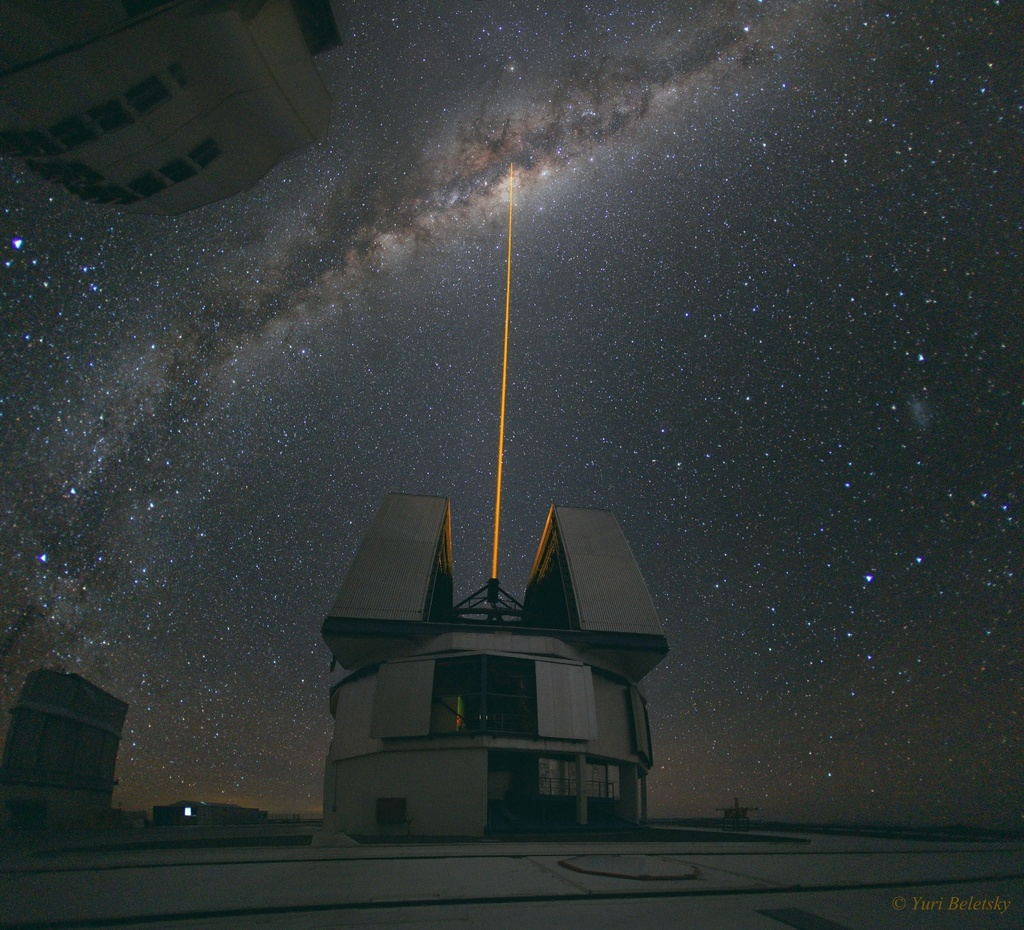
\includegraphics[width=0.55\textwidth]{img/galactic-center}
        \caption{A laser strike at the Galactic Center (Yuri Beletsky)}
        \label{fig:galactic-center}
    \end{figure}
\end{frame}

\begin{frame}
    \frametitle{Introduction}
    \framesubtitle{Galactic center}
    \begin{itemize}
        \item Rotational center of the Milky Way.
        \item Strong evidence about the existence of a SMBH.
            \item Astronomical radio source (Sagittarius A)
            \item BH diameter $\approx$ 0.3 AU
            \begin{itemize}
                \item $1 AU \approx 149\cdot10^{6} km$ 
            \end{itemize}
            \item BH mass $\approx 4\cdot 10^{6} M_{\odot}$
            \begin{itemize}
                \item $M_{\odot} \approx 1.9\cdot 10^{30} kg$
            \end{itemize}
    \end{itemize}
\end{frame}

\begin{frame}
    \frametitle{Introduction}
    \framesubtitle{The puzzle}
    \begin{itemize}
        \item Population of young massive stars (~5 Myr) orbiting a fraction of a pc.
        \begin{itemize}
            \item $1 pc \approx 3.1\cdot 10^{13} km$
        \end{itemize}
        \item Their existence is a puzzle.
        \begin{itemize}
            \item Tidal field prevents star formation.
            \item Isotropic orbits (S-stars).
            \item Many stars lie on a single plane.
        \end{itemize}
        \item Big question: \blue{"How this disc was formed?"}
    \end{itemize}
\end{frame}

\begin{frame}
    \frametitle{Introduction}
    \framesubtitle{Formation theories}
    Two main theories:
    \begin{enumerate}
        \item Inside the accretion disc, exceeding the tidal limit.
        \item Outside the GC but migrated to the disc.
    \end{enumerate}
\end{frame}
